\chapter{Các hướng đã thử}
\label{app:A}

Phụ lục này trình bày, theo thứ tự thực hiện, các hướng đã thử trước khi chọn phương pháp đề xuất, với phần tóm tắt ở Mục~\ref{sec:6.10}. Trong các bảng, S1 là mô hình tinh chỉnh có giám sát, dùng làm mốc so sánh; S2 là mô hình mô tả phần tử; CE2-S2 là mô hình học thêm có giám sát; MIN-DESC (MIN) là mô hình sau giai đoạn học ưu tiên; Base là mô hình gốc và Trần là câu chuẩn.

\section{Mô tả phần tử trước khi viết câu}\label{sec:A.1}

\subsection{Thiết kế}\label{sec:A.1.1}

Hướng đầu tiên dạy mô hình mô tả phần tử cần chạm trước rồi mới viết câu, thay vì sinh thẳng câu từ ảnh. Mô hình được huấn luyện theo cách này gọi là mô hình mô tả phần tử. Chuỗi mà mô hình cần sinh gồm hai phần, như ở khối dưới đây.

\begin{center}\small
\begin{tabularx}{\textwidth}{@{}lX@{}}
\toprule
dòng mô tả phần tử & \code{<desc>} vai trò | tên | \code{<point>}$x,y$\code{</point>} | dấu hiệu phân biệt \code{</desc>} \\
phần câu & câu hướng dẫn \\
\bottomrule
\end{tabularx}
\end{center}

Lúc đánh giá, dòng mô tả bị cắt bỏ và mô hình định vị chỉ nhận câu hướng dẫn, nên nếu điểm tăng thì lý do nằm ở hành vi của mô hình sinh câu. Thiết kế dựa trên ba căn cứ. Thứ nhất, dạng lỗi đã đo được chủ yếu là câu mơ hồ (Chương~\ref{chap:1}), nên dòng mô tả có một ô ghi dấu hiệu phân biệt. Thứ hai, hai dòng Shikra trong Bảng~\ref{tab:1.1} cho kết quả âm khi bước trung gian là văn xuôi và dương khi bước trung gian có tọa độ, nên dòng mô tả gồm bốn ô cố định và bắt buộc có tọa độ. Thứ ba, tọa độ chạm của người thật có sẵn trong dữ liệu, nên nhãn tọa độ sạch 100\% mà không tốn chi phí dựng. Thiết kế còn có mục thứ hai, tức phạt mô hình khi xác suất của dòng mô tả trỏ đúng phần tử không vượt xác suất của dòng mô tả trỏ sang phần tử lân cận ít nhất một khoảng lề, là phần mà Widget Captioning~\cite{widgetcap} chưa xử lý. Mục này chưa được thực hiện vì mục thứ nhất, tức bản thân dòng mô tả, chưa cho thấy tác dụng (Mục~\ref{sec:A.1.3}).

\subsection{Các cấu hình của thiết kế so sánh ban đầu}\label{sec:A.1.2}

Thiết kế so sánh ban đầu gồm bảy cấu hình, dùng chung dữ liệu, mô hình gốc, siêu tham số và tập kiểm tra (Bảng~\ref{tab:A.1}).

\begin{table}[htbp]
\centering\small
\caption[Các cấu hình của thiết kế so sánh ban đầu.]{Các cấu hình của thiết kế so sánh ban đầu. Ba cấu hình cuối không cần huấn luyện.}\label{tab:A.1}
\setlength{\tabcolsep}{4pt}
\begin{tabularx}{\textwidth}{@{}>{\raggedright\arraybackslash\hsize=0.62\hsize}X>{\raggedright\arraybackslash\hsize=0.95\hsize}X>{\raggedright\arraybackslash\hsize=1.43\hsize}X@{}}
\toprule
\textbf{Cấu hình} & \textbf{Chuỗi phải sinh ra hoặc cách chạy} & \textbf{Vai trò} \\
\midrule
Tinh chỉnh có giám sát (S1) & chỉ câu hướng dẫn (2 hạt giống) & mốc so sánh \\
Mô tả phần tử (S2) & dòng mô tả thật + câu (2 hạt giống) & phép so sánh chính của thiết kế ban đầu, kiểm tác dụng của việc mô tả phần tử trước \\
Mô tả giả (S2r) & dòng mô tả giả khớp độ dài + câu & loại trừ khả năng điểm tăng chỉ do chuỗi phải sinh ra dài thêm \\
Mô tả không có tọa độ (S2-nopoint) & dòng mô tả bỏ tọa độ + câu & tách phần đóng góp của tọa độ \\
Danh sách phần tử lúc chạy (B-infer) & trọng số S1, danh sách phần tử đưa vào đầu vào lúc chạy & so huấn luyện với việc chỉ cung cấp thông tin lúc chạy \\
Mô hình gốc (Base) & mô hình gốc, không tinh chỉnh & đo phần cải thiện do bản thân việc tinh chỉnh \\
Câu chuẩn (Trần) & câu chuẩn đưa thẳng đi đánh giá & ngưỡng tối đa của độ đo \\
\bottomrule
\end{tabularx}
\end{table}

Đại lượng quan tâm là $\Delta$ = S2 $-$ S1, tính trên trung bình hai hạt giống của mỗi mô hình. Hai lượt huấn luyện mô hình tinh chỉnh có giám sát chỉ khác nhau ở hạt giống, nên chênh lệch giữa chúng cho biết điểm số dao động bao nhiêu khi chỉ huấn luyện lại mà không có can thiệp nào. Bốn cấu hình không được chạy, gồm hạt giống thứ hai của mô hình mô tả phần tử, cấu hình mô tả giả, cấu hình mô tả không có tọa độ và cấu hình chỉ đưa danh sách phần tử vào lúc chạy (lý do ở Bảng~\ref{tab:6.13}). Do thiếu hạt giống thứ hai của mô hình mô tả phần tử, $\Delta$ không tính đủ được theo định nghĩa trên.

\subsection{Kết quả}\label{sec:A.1.3}

Mô hình mô tả phần tử đạt 57,2\%, thấp hơn mô hình tinh chỉnh có giám sát 1,93 điểm ở hạt giống 101 và 2,44 điểm ở hạt giống 202 (Bảng~\ref{tab:6.8}); khoảng tin cậy của cả hai chênh lệch đều nằm dưới 0. Theo tiêu chí ở Mục~\ref{sec:4.8}, đây là kết quả âm, dù chưa đủ để kết luận rằng việc mô tả phần tử trước luôn gây hại. Kết quả âm này giữ nguyên khi đánh giá lại bằng mô hình định vị thứ hai (Mục~\ref{sec:5.9}). Mô hình vẫn hơn mô hình gốc 9,59 điểm, nên việc thêm dòng mô tả không làm mất tác dụng của việc tinh chỉnh.

Chúng tôi đã kiểm ba cách giải thích thay thế và không cách nào giải thích được chênh lệch. Ba cách đó là độ dài câu, nhóm ứng dụng, và tên ghi trong dòng mô tả bị sai do lỗi nhận dạng chữ.

\subsubsection{Chia nhóm theo việc có sinh dòng mô tả hay không}\label{sec:A.1.3.1}

\begin{table}[htbp]
\centering\small
\caption{Điểm chia theo việc mô hình mô tả phần tử (S2) có sinh dòng mô tả hay không.}\label{tab:A.2}
\begin{tabular}{@{}lrrrr@{}}
\toprule
\textbf{Nhóm} & \textbf{n} & \textbf{S1} & \textbf{S2} & \textbf{$\Delta$} \\
\midrule
Có sinh dòng mô tả & 4.138 & 62,2 & 60,8 & -1,38 [$-$2,54; $-$0,19] \\
Không sinh dòng mô tả & 325 & 19,7 & 10,8 & -8,92 [$-$12,57; $-$5,25] \\
\bottomrule
\end{tabular}
\end{table}

Theo Bảng~\ref{tab:A.2}, nhóm 325 bước mà mô hình mô tả phần tử bỏ qua dòng mô tả chỉ gồm 7,3\% số bước nhưng chiếm 34\% toàn bộ chênh lệch. Ở nhóm này mô hình phần lớn đoán sai loại thao tác, trong khi câu chuẩn vẫn đạt 68,3\%, tức các bước này vẫn giải được. Mô hình gốc gọi đúng loại thao tác ở 83,4\% số bước trong nhóm, mô hình tinh chỉnh có giám sát ở 55,1\% và mô hình mô tả phần tử ở 38,8\%. Như vậy chính việc tinh chỉnh đã làm lệch xu hướng chọn loại thao tác, và việc thêm dòng mô tả khuếch đại độ lệch ấy. Chúng tôi nghi đây là một lỗi tắt học từ dữ liệu, vì tập huấn luyện chỉ gắn dòng mô tả cho bước chạm, nên mô hình có thể học quy tắc “đã viết dòng mô tả thì là chạm”. Giả thuyết này chưa được kiểm vì cấu hình mô tả không có tọa độ đã bị hủy. Nhóm này được định nghĩa bằng hành vi của chính mô hình mô tả phần tử, nên việc mô hình này kém trên nhóm một phần là hệ quả của cách chia nhóm. Dù vậy, mô hình tinh chỉnh có giám sát cũng chỉ đạt 19,7\% trên cùng nhóm.

\subsubsection{Ảnh hưởng hai chiều của dòng mô tả}\label{sec:A.1.3.2}

\begin{table}[htbp]
\centering\small
\caption[Điểm theo trạng thái dòng mô tả do mô hình mô tả phần tử (S2) tự sinh.]{Điểm theo trạng thái dòng mô tả do mô hình mô tả phần tử (S2) tự sinh. Cột Trần là điểm của câu chuẩn trên chính nhóm đó.}\label{tab:A.3}
\setlength{\tabcolsep}{3pt}
\begin{tabular}{@{}llrrrrr@{}}
\toprule
\textbf{Tên} & \textbf{Tọa độ} & \textbf{n} & \textbf{Base} & \textbf{S1} & \textbf{S2} & \textbf{Trần} \\
\midrule
đúng & trúng & 1.871 & 69,0 & 81,4 & 87,1 & 86,6 \\
đúng & trượt & 184 & 23,4 & 25,5 & 26,1 & 31,0 \\
sai & trúng & 452 & 41,4 & 56,4 & 57,5 & 72,8 \\
sai & trượt & 738 & 24,4 & 30,8 & 5,6 & 66,3 \\
không sinh dòng mô tả &  & 228 & 25,9 & 20,6 & 9,6 & 70,6 \\
\bottomrule
\end{tabular}
\end{table}

Bảng~\ref{tab:A.3} chia các bước được đánh giá theo việc dòng mô tả do chính mô hình mô tả phần tử sinh ra có đúng tên và tọa độ hay không. Khi đúng cả hai, mô hình đạt 87,1\%, hơn mô hình tinh chỉnh có giám sát 5,7 điểm và vượt cả câu chuẩn trên nhóm đó. Khi sai cả hai, mô hình chỉ còn 5,6\%, dưới cả mức ngưỡng tối thiểu của độ đo (câu chung chung không nói phần tử nào đạt 12,0\%, Mục~\ref{sec:5.6}), trong khi câu chuẩn vẫn đạt 66,3\% trên 738 bước ấy. Ở nhóm này mô hình đã chọn một phần tử sai rồi viết câu khẳng định về phần tử đó, còn mô hình tinh chỉnh có giám sát viết câu chung chung nên vẫn có cơ hội trúng. Dòng mô tả vì vậy khuếch đại kết quả theo cả hai chiều, và đây là căn cứ của giai đoạn học ưu tiên (Mục~\ref{sec:A.2.1}).

\section{Học ưu tiên trên dòng mô tả}\label{sec:A.2}

\subsection{Thiết kế}\label{sec:A.2.1}

Kết quả của mô hình mô tả phần tử cho thấy độ chính xác của dòng mô tả đang là nguyên nhân hạn chế kết quả chung (Mục~\ref{sec:A.1.3.2}), trong khi học có giám sát thuần chỉ nâng xác suất của chuỗi đúng mà không hạ xác suất của chuỗi sai gần kề. Giai đoạn học ưu tiên trên dòng mô tả (gọi tắt là giai đoạn học ưu tiên, trong bảng là MIN-DESC) vì vậy học tiếp từ trọng số đã huấn luyện của mô hình mô tả phần tử thêm 800 bước cập nhật, với một mục tiêu ưu tiên trên các cặp quy chiếu tối thiểu có dạng như sau.

\begin{center}\small
\begin{tabular}{@{}ll@{}}
\toprule
vế được chọn & \code{<desc>}mô tả trỏ đúng phần tử\code{</desc>} $+$ \code{\textbackslash n} $+$ câu \\
vế bị loại & \code{<desc>}mô tả trỏ sai phần tử\code{</desc>} $+$ \code{\textbackslash n} $+$ đúng câu đó \\
\bottomrule
\end{tabular}
\end{center}

Hai vế chỉ khác nhau ở dòng mô tả, nên số hạng ưu tiên chỉ giảm được khi mô hình chọn đúng phần tử. Dòng mô tả trỏ sai là mô tả của một phần tử có thật, cùng vai trò, nằm gần phần tử cần chạm; cách dựng 22.854 cặp nằm ở Mục~\ref{sec:3.7}. Hàm mục tiêu thuộc họ tối ưu theo ưu tiên dạng tỉ số odds (ORPO), không cần mô hình tham chiếu đóng băng.

Để tách phần của mục tiêu ưu tiên khỏi phần của việc học thêm, mô hình học thêm có giám sát (CE2-S2) học có giám sát thuần trên vế được chọn của các cặp ấy, cùng điểm xuất phát và số bước. Đại lượng chính là hiệu ghép cặp $\Delta$\_thành phần = MIN-DESC $-$ CE2-S2, tính trên cùng các bước của tập kiểm tra (Mục~\ref{sec:4.8}). Tập cặp chỉ chứa bước chạm, nên thiệt hại ở bước không chạm được đo riêng (Mục~\ref{sec:A.2.2.4}).

\subsection{Kết quả}\label{sec:A.2.2}

\subsubsection{Độ chính xác của dòng mô tả}\label{sec:A.2.2.1}

Bảng~\ref{tab:A.4} đối chiếu thẳng dòng mô tả do mô hình tự sinh với nhãn chuẩn của tập kiểm tra, không cần gọi mô hình định vị.

\begin{table}[htbp]
\centering\small
\caption{Độ chính xác của dòng mô tả trên 3.473 bước có tên đúng để đối chiếu, chỉ tính các bước có mặt trong kết quả của cả ba mô hình.}\label{tab:A.4}
\setlength{\tabcolsep}{4pt}
\begin{tabularx}{\textwidth}{@{}>{\raggedright\arraybackslash\hsize=1.00\hsize}Xrrrr@{}}
\toprule
\textbf{Mô hình} & \textbf{Sinh dòng mô tả} & \textbf{Tên đúng} & \textbf{Tọa độ đúng} & \textbf{Cả hai đúng} \\
\midrule
Mô tả phần tử (S2) & 93,4\% & 59,2\% & 66,9\% & 53,9\% \\
Học thêm có giám sát (CE2-S2) & 99,6\% & 66,2\% & 71,2\% & 59,8\% \\
Học ưu tiên (MIN-DESC) & 99,6\% & 67,0\% & 71,8\% & 60,6\% \\
\bottomrule
\end{tabularx}
\end{table}

So với mô hình mô tả phần tử, tỉ lệ đúng cả tên lẫn tọa độ sau giai đoạn học ưu tiên tăng 6,77 điểm. Mô hình học thêm có giám sát cũng đạt 5,93 điểm trong mức tăng ấy, nên phần riêng của mục tiêu ưu tiên chỉ là 0,84 điểm, và 87,7\% mức tăng đến từ chính việc học thêm.

\subsubsection{Executability và đại lượng chính}\label{sec:A.2.2.2}

Sau giai đoạn học ưu tiên, mô hình đạt 60,0\%, còn mô hình học thêm có giám sát đạt 59,4\% (Bảng~\ref{tab:6.1}). Đại lượng chính $\Delta$\_thành phần bằng +0,63 điểm, khoảng tin cậy 95\% là [+0,16; +1,10] và p = 0,011 (Bảng~\ref{tab:6.8}). Khoảng tin cậy không chứa 0, nhưng mức này chỉ bằng 1,4 lần độ lệch chuẩn giữa hai hạt giống (0,46 điểm, Mục~\ref{sec:6.7}), tức chưa vượt rõ mức dao động khi chỉ huấn luyện lại với hạt giống khác. Vì vậy chúng tôi không gọi đây là tác dụng của mục tiêu ưu tiên. MIN-DESC hơn mô hình mô tả phần tử 2,87 điểm, nhưng 2,24 điểm trong đó đã có ở mô hình học thêm có giám sát, tức 78\% mức tăng thuộc về bản thân việc học thêm. So với hạt giống 101 của mô hình tinh chỉnh có giám sát, MIN-DESC chỉ hơn 0,94 điểm và mô hình học thêm hơn 0,31 điểm, đều có khoảng tin cậy phủ 0. Giai đoạn học ưu tiên vì vậy chủ yếu sửa lại thiệt hại do chính dòng mô tả gây ra, rồi tăng thêm một mức nhỏ so với mô hình tinh chỉnh có giám sát.

\subsubsection{Biến thể lấy vế bị loại theo chính sách}\label{sec:A.2.2.3}

Ngoài nguồn dựng bằng luật (cửa sổ 80 đến 350 điểm ảnh quanh phần tử cần chạm), chúng tôi thử lấy vế bị loại theo chính sách (\emph{on-policy}), tức lấy chính phần tử mà mô hình gọi nhầm. Hướng này dừng trước khi huấn luyện, vì cho mô hình sinh dòng mô tả trên 14.000 màn huấn luyện chỉ thu được 459 cặp hợp lệ, tức 3,3\% số màn. Trên 3.246 bước gọi sai tên, khoảng cách từ phần tử bị gọi nhầm tới phần tử cần chạm có trung vị 351 điểm ảnh, và cửa sổ 80 đến 350 điểm ảnh loại mất 76,5\% số bước này. Lỗi trong dòng mô tả vì vậy rơi vào hai cực. Mô hình hoặc gọi đúng phần tử bằng tên khác, hoặc nhìn sang hẳn một vùng khác của màn hình, và hiếm khi lẫn giữa hai nút cạnh nhau như biến thể này giả định. Vế bị loại dựng bằng luật vì thế phải tự tạo ra dạng lẫn giữa hai phần tử gần nhau mà mô hình ít khi tự mắc. Cách dựng này là nguồn còn dùng được sau phép đo trên, không phải lựa chọn thiết kế từ đầu.

\subsubsection{Thiệt hại đo được ở bước không chạm}\label{sec:A.2.2.4}

\begin{table}[htbp]
\centering\small
\caption{Khớp loại thao tác trên mẫu 400 bước không chạm (cuộn 96, chờ 86, gõ chữ 82, mở ứng dụng 81, quay lại 55), đánh giá với biến thể nghiêm ngặt của điều kiện khớp loại thao tác.}\label{tab:A.5}
\begin{tabular}{@{}lrr@{}}
\toprule
\textbf{Mô hình} & \textbf{Khớp loại thao tác} & \textbf{$\Delta$ so với S2} \\
\midrule
Mô tả phần tử (S2) & 83,5\% & – \\
Học thêm có giám sát (CE2-S2) & 63,0\% & -20,50 \\
Học ưu tiên (MIN-DESC) & 63,8\% & -19,75 \\
\bottomrule
\end{tabular}
\end{table}

Đánh giá ở bước không chạm (Mục~\ref{sec:5.13}) cho thấy sau giai đoạn học ưu tiên, mô hình kém đi rất nhiều ở nhóm bước này (Bảng~\ref{tab:A.5}). Mức giảm tập trung ở cuộn ($-$43,8), quay lại ($-$36,4) và gõ chữ ($-$29,2), ba loại thao tác mà câu chuẩn không nhắc tên phần tử nào; hai loại chờ và mở ứng dụng không giảm, nhưng chỉ vì phép chuẩn hoá loại thao tác xếp động từ “mở” vào lớp chạm. Mô hình học thêm có giám sát giảm gần như ngang bảng ($-$20,50 so với $-$19,75), nên mức giảm gắn với việc học thêm trên dữ liệu chỉ gồm bước chạm, không phải với mục tiêu ưu tiên. Executability chỉ đánh giá bước chạm nên không thấy mức giảm này.

\subsection{Tìm chỗ nghẽn của cách mô tả phần tử trước}\label{sec:A.2.3}

Cách chia nhóm dựa trên hành vi của chính mô hình được đo. Hai nhóm khác nhau nhiều về độ khó, nên chỉ phép so sánh ghép cặp bên trong một nhóm là hợp lệ. Bảng~\ref{tab:A.6} chia 3.473 bước có tên đúng để đối chiếu theo việc dòng mô tả của MIN-DESC trỏ đúng phần tử (tên khớp và tọa độ nằm trong dung sai 14\%) hay trỏ sai.

\begin{table}[htbp]
\centering\small
\caption[Điểm của mô hình sau giai đoạn học ưu tiên (MIN-DESC) và mô hình tinh chỉnh có giám sát (S1) trên 3.473 bước có tên đúng để đối chiếu, chia theo việc dòng mô tả của MIN-DESC trỏ đúng hay trỏ sai phần tử.]{Điểm của mô hình sau giai đoạn học ưu tiên (MIN-DESC) và mô hình tinh chỉnh có giám sát (S1) trên 3.473 bước có tên đúng để đối chiếu, chia theo việc dòng mô tả của MIN-DESC trỏ đúng hay trỏ sai phần tử. Cột Trần là điểm của câu chuẩn trên chính nhóm đó.}\label{tab:A.6}
\begin{tabular}{@{}lrrrrr@{}}
\toprule
\textbf{Nhóm} & \textbf{n} & \textbf{MIN-DESC} & \textbf{S1} & \textbf{$\Delta$ ghép cặp} & \textbf{Trần} \\
\midrule
Trỏ đúng phần tử & 2.106 (60,6\%) & 87,1 & 78,3 & +8,83 & 86,3 \\
Trỏ sai phần tử & 1.367 (39,4\%) & 21,8 & 32,9 & -11,12 & 61,4 \\
\bottomrule
\end{tabular}
\end{table}

Khi dòng mô tả trỏ đúng phần tử, MIN-DESC hơn mô hình tinh chỉnh có giám sát 8,83 điểm và vượt cả ngưỡng tối đa của câu chuẩn trên nhóm đó; khi dòng mô tả trỏ sai, MIN-DESC thấp hơn 11,12 điểm. Hai chiều gần như triệt tiêu nhau, chỉ còn lại mức +0,94 điểm không có ý nghĩa thống kê (Mục~\ref{sec:A.2.2}). Như vậy việc mô tả phần tử trước có tác dụng đúng như giả thuyết, nhưng chỉ trên 60,6\% số bước mà dòng mô tả trỏ trúng.

\textbf{Ngưỡng tối đa lý thuyết khi bù được phần thiệt ở các bước mô tả sai.} Giả sử ở mỗi bước mà dòng mô tả trỏ sai, MIN-DESC cho đúng kết quả của mô hình tinh chỉnh có giám sát. Khi đó điểm trên 3.473 bước có tên đúng để đối chiếu sẽ là 65,8\% thay vì 61,4\% thực đo, tức cao hơn mô hình tinh chỉnh có giám sát 5,4 điểm. Mức này không đạt được ở khâu suy luận bằng một quy tắc chọn câu ở từng bước, tức quyết định lấy câu của MIN-DESC hay câu của mô hình tinh chỉnh có giám sát. Một quy tắc hoàn hảo, biết trước dòng mô tả trỏ đúng hay sai, cho 63,5\% trên toàn bộ 4.463 bước, nhưng bảy quy tắc thực tế đã thử chỉ cho 60,0 đến 60,3\%, không khác biệt rõ so với mức 60,0\% của MIN-DESC. Chỗ nghẽn này vì vậy phải được sửa ở khâu huấn luyện.

\begin{table}[htbp]
\centering\small
\caption[Phân rã toàn bộ 4.463 bước theo trạng thái dòng mô tả của MIN-DESC (cột MIN).]{Phân rã toàn bộ 4.463 bước theo trạng thái dòng mô tả của MIN-DESC (cột MIN). Cột cuối là phần dư địa tới mức câu chuẩn mà mỗi nhóm đóng góp, tính bằng điểm trên toàn tập bước được đánh giá.}\label{tab:A.7}
\setlength{\tabcolsep}{3pt}
\begin{tabularx}{\textwidth}{@{}>{\raggedright\arraybackslash\hsize=1.00\hsize}Xrrrrrr@{}}
\toprule
\textbf{Nhóm} & \textbf{n} & \textbf{\%} & \textbf{MIN} & \textbf{S1} & \textbf{Trần} & \textbf{Dư địa} \\
\midrule
tên đúng, tọa độ đúng & 2.082 & 46,7 & 87,1 & 78,2 & 86,3 & -0,36 \\
tên đúng, tọa độ sai & 220 & 4,9 & 26,4 & 27,7 & 32,3 & +0,29 \\
tên sai, tọa độ đúng & 411 & 9,2 & 57,2 & 53,0 & 73,0 & +1,46 \\
không sinh dòng mô tả & 15 & 0,3 & 0,0 & 0,0 & 60,0 & +0,20 \\
tên sai, tọa độ sai & 745 & 16,7 & 3,6 & 25,8 & 64,4 & +10,15 \\
không có tên để đối chiếu & 990 & 22,2 & 55,3 & 54,4 & 73,0 & +3,94 \\
\textbf{Tổng} & \textbf{4.463} &  & \textbf{60,0} & \textbf{59,1} & \textbf{75,7} & \textbf{+15,7} \\
\bottomrule
\end{tabularx}
\end{table}

Theo Bảng~\ref{tab:A.7}, nhóm đúng cả tên lẫn tọa độ chiếm 46,7\% số bước và không còn dư địa, vì ở nhóm này mô hình đã vượt ngưỡng tối đa của câu chuẩn. Phần lớn dư địa còn lại (63\%) nằm ở nhóm sai cả tên lẫn tọa độ. Trên nhóm này MIN-DESC chỉ đạt 3,6\% và mô hình tinh chỉnh có giám sát đạt 25,8\%, trong khi câu chuẩn đạt 64,4\%, nên đây không phải nhóm bước bất khả thi.

\section{Chọn phần tử trong danh sách ứng viên}\label{sec:A.3}

\subsection{Thiết kế}\label{sec:A.3.1}

Phân tích ở Mục~\ref{sec:A.2.3} cho thấy phần lớn dư địa còn lại của MIN-DESC nằm ở những bước mà dòng mô tả sai cả tên lẫn tọa độ. Vì vậy, thay vì để mô hình tự viết dòng mô tả, chúng tôi cho mô hình chọn phần tử trong danh sách lấy từ chính màn hình; mô hình huấn luyện theo cách này gọi là mô hình chọn ứng viên. Căn cứ là ba con số đo được trước khi huấn luyện. Tên đúng có mặt trong chữ OCR hoặc cây trợ năng ở 99,7\% số bước. Ở 80,2\% số bước có một ứng viên vừa khớp tên vừa nằm trong dung sai, so với 59,9\% của dòng mô tả tự sinh. Ở 67,7\% số bước mà MIN-DESC gọi sai tên, tên đúng đã nằm sẵn trong 24 dòng OCR của câu nhắc nhưng không kèm vị trí.

\textbf{Cách làm.} Câu nhắc thay 24 dòng OCR bằng danh sách ứng viên ở Mục~\ref{sec:3.8}. Chuỗi đích mở đầu bằng một thẻ chọn, là bản chép nguyên văn một dòng trong danh sách hoặc thẻ \code{none}, rồi mới tới câu; thẻ này được cắt bỏ trước khi đánh giá. Phần được đo là việc chọn tường minh, tức mô hình ghi rõ ứng viên mình chọn ngay trong chuỗi đích.

\textbf{Điều kiện thí nghiệm.} Mô hình chọn ứng viên khác mô hình tinh chỉnh có giám sát (S1) và MIN-DESC ở ba biến. Ngữ cảnh dài 3072 thay vì 2560 token để chứa danh sách ứng viên (mẫu dài nhất 2.017 token cộng danh sách dài nhất 1.012 token), số lượt duyệt chỉ còn một (4.036 bước) do giới hạn tài nguyên, và đầu vào có thêm danh sách ứng viên. Vì vậy điểm của mô hình này không thể đem trừ thẳng cho điểm của hai mô hình kia. Đại lượng hợp lệ là hiệu ghép cặp $\Delta$\_chọn với một cấu hình đối chứng nhận cùng danh sách ứng viên ở đầu vào nhưng chuỗi đích chỉ có câu, còn các tham số khác giữ như Bảng~\ref{tab:4.1}. Thiết kế ban đầu gồm sáu lượt huấn luyện (ba cấu hình, mỗi cấu hình hai hạt giống), nhưng năm lượt sau chỉ được chạy nếu lượt đầu cho độ chính xác chọn hơn rõ tỉ lệ 60,6\% dòng mô tả trỏ đúng phần tử của MIN-DESC. Độ chính xác chọn là tỉ lệ thẻ chọn trúng phần tử cần chạm (tên khớp, tọa độ trong dung sai 14\%) trên những bước mà danh sách có chứa phần tử ấy, tức có ứng viên đúng, đo trên 1.400 bước chạm đầu của tập kiểm tra.

\subsection{Kết quả}\label{sec:A.3.2}

Mô hình chọn ứng viên được huấn luyện với hạt giống 101 trên 64.567 mẫu của Mục~\ref{sec:3.8}.

\subsubsection{Độ chính xác chọn và executability}\label{sec:A.3.2.1}

Trên 1.400 bước dùng làm tiêu chí, 1.008 bước có ứng viên đúng và thẻ chọn trúng ở 580 bước, cho độ chính xác chọn 57,54\%, thấp hơn mức 60,6\% của MIN-DESC, nên năm lượt còn lại không được chạy. Từ đây, 1.400 bước này được gọi là \emph{mẫu phát triển}, còn 3.062 bước còn lại chỉ dùng để đọc kết quả. Độ chính xác chọn cũng không phải đại lượng tốt để ra quyết định, vì cũng như cột “có đáp án” của SQuAD 2.0~\cite{rajpurkar2018}, đại lượng này chỉ đếm những bước có đáp án. Khi ép mô hình luôn chọn, độ chính xác chọn lên 69,05\%, nhưng tỉ lệ thẻ đúng trên cả mẫu phát triển giảm từ 63,43\% xuống 49,71\%.

Trên 4.463 bước chạm, mô hình chọn ứng viên đạt 56,1\%, khoảng tin cậy [54,2; 58,0] (bootstrap theo 1.091 cụm), với tỉ lệ khớp loại thao tác 90,9\% và tỉ lệ trúng ô Voronoi thuần 57,4\%. Điểm trên mẫu phát triển (55,4\%) và trên phần còn lại (56,5\%) gần nhau. Mô hình hơn mô hình gốc (chưa tinh chỉnh) 8,54 điểm (731 bước chỉ mô hình chọn ứng viên đúng, 350 bước chỉ mô hình gốc đúng, kiểm định McNemar cho p < 0,001), và chỉ phép so sánh này đọc được thành kết luận. Cấu hình đối chứng nhận cùng danh sách ứng viên nằm trong năm lượt không được chạy, nên không tách được đóng góp riêng của việc chọn tường minh hay của danh sách ứng viên.

\subsubsection{Hành vi chọn và từ chối chọn}\label{sec:A.3.2.2}

\begin{table}[htbp]
\centering\small
\caption[Mô hình chọn ứng viên, chia theo việc danh sách có ứng viên đúng và việc mô hình có đưa ra lựa chọn hay không.]{Mô hình chọn ứng viên, chia theo việc danh sách có ứng viên đúng và việc mô hình có đưa ra lựa chọn hay không. Hàng đầu và hàng cuối là hành vi đúng, hai hàng giữa là hai dạng lỗi.}\label{tab:A.8}
\setlength{\tabcolsep}{4pt}
\begin{tabularx}{\textwidth}{@{}llrrrr@{}}
\toprule
\textbf{Có ứng viên đúng} & \textbf{Mô hình} & \textbf{n} & \textbf{\% tập} & \textbf{Exec.} & \textbf{Khớp thao tác} \\
\midrule
có & \textbf{chọn} & 2.326 & 52,1 & \textbf{71,4 [69,5; 73,2]} & 99,1 \\
có & \textbf{từ chối (sai)} & 872 & 19,5 & \textbf{23,7 [21,0; 26,7]} & 71,2 \\
không & chọn (sai) & 264 & 5,9 & 37,5 & 99,6 \\
không & \textbf{từ chối (đúng)} & 1.001 & 22,4 & 53,8 & 86,6 \\
\bottomrule
\end{tabularx}
\end{table}

Khi danh sách có ứng viên đúng và mô hình đưa ra lựa chọn, điểm đạt 71,4\%, cao hơn mọi mô hình đã huấn luyện và chỉ kém câu chuẩn 4,3 điểm, nên cơ chế chọn hoạt động đúng. Thiệt hại nằm ở hàng thứ hai, gồm 872 bước (27,3\% số bước có ứng viên đúng) mà mô hình từ chối chọn dù đáp án nằm sẵn trong danh sách, và nhóm này chỉ đạt 23,7\%. Tỉ lệ từ chối nhầm này lặp lại mức 27,1\% đo độc lập trên mẫu phát triển. Trên toàn tập, mô hình từ chối chọn ở 41,97\% số bước. Nếu nhóm từ chối nhầm đạt mức 68,0\% của nhóm đưa ra lựa chọn, điểm toàn tập sẽ là 65,4\%, tức +9,3 điểm; đây là ngưỡng tối đa ước lượng cùng dạng với con số +5,4 ở Mục~\ref{sec:A.2.3}, không phải kết quả đã chạy.

\textbf{Dấu hiệu đi kèm việc từ chối chọn.} Câu mang động từ không phải chạm chiếm 28,3\% số bước từ chối chọn, so với 0,97\% ở bước đưa ra lựa chọn, giống hiện tượng lẫn loại thao tác ở Mục~\ref{sec:A.1.3.1}. Sai số của mô hình định vị ở nhóm từ chối chọn có trung vị 19,9\% bề ngang màn, so với 0,78\% ở nhóm còn lại, tức mô hình nhìn sang vùng khác của màn như dạng lỗi lưỡng cực ở Mục~\ref{sec:A.2.2.3}. Danh sách càng dài thì mô hình càng hay từ chối chọn (Bảng~\ref{tab:A.9}), nhưng màn nhiều phần tử cũng là màn khó hơn, nên đây chỉ là tương quan.

\begin{table}[htbp]
\centering\small
\caption[Tỉ lệ từ chối chọn và executability theo số dòng trong danh sách, chỉ tính bước có ứng viên đúng.]{Tỉ lệ từ chối chọn và executability theo số dòng trong danh sách, chỉ tính bước có ứng viên đúng.}\label{tab:A.9}
\begin{tabular}{@{}lrrr@{}}
\toprule
\textbf{Số dòng trong danh sách} & \textbf{n} & \textbf{Từ chối chọn} & \textbf{Exec.} \\
\midrule
1 đến 5 & 178 & 18,5\% & 70,8 \\
6 đến 10 & 363 & 15,7\% & 70,5 \\
11 đến 20 & 826 & 25,9\% & 60,3 \\
21 đến 39 & 1.036 & 29,3\% & 55,6 \\
40 (mức tối đa) & 795 & 33,2\% & 51,8 \\
\bottomrule
\end{tabular}
\end{table}

Tỉ lệ từ chối chọn cũng cao hơn khi ứng viên đúng nằm giữa danh sách (31,4\%, so với 27,2\% ở phần đầu và 24,3\% ở phần cuối), giống hiện tượng Liu và cộng sự~\cite{liu2024lost} mô tả cho ngữ cảnh dài. Đây là quan sát chưa qua kiểm định, và vị trí trong danh sách có tương quan với độ dài danh sách.

\subsubsection{Tiên nghiệm của nhãn từ chối chọn trong tập huấn luyện}\label{sec:A.3.2.3}

\begin{table}[htbp]
\centering\small
\caption[Tỉ lệ thẻ \code{none} theo bốn mẫu số.]{Tỉ lệ thẻ \code{none} theo bốn mẫu số. Mô hình phát \code{none} nhiều hơn tỉ lệ đúng trên loại bước bị đánh giá, và ít hơn tỉ lệ gặp trên toàn tập huấn luyện.}\label{tab:A.10}
\begin{tabular}{@{}lr@{}}
\toprule
\textbf{Mẫu số} & \textbf{Tỉ lệ \code{none}} \\
\midrule
Toàn bộ tập huấn luyện (64.567 mẫu) & 54,78\% \\
Chỉ bước chạm của tập huấn luyện (41.191) & 29,12\% \\
Bước chạm của tập kiểm tra, tỉ lệ đúng (4.463) & 28,34\% \\
Tỉ lệ mô hình phát ra trên tập kiểm tra & 41,97\% \\
\bottomrule
\end{tabular}
\end{table}

Tỉ lệ mô hình phát ra nằm giữa tỉ lệ đúng trên bước chạm và tỉ lệ trên toàn tập huấn luyện, và gần tỉ lệ toàn tập hơn. Vì mọi bước không chạm đều mang thẻ \code{none} (Mục~\ref{sec:3.8}), hơn một nửa số mẫu dạy mô hình phát thẻ này. Cách giải thích của chúng tôi là mô hình học tỉ lệ nền ấy, tức tiên nghiệm của nhãn, rồi mang sang bước chạm, là loại bước duy nhất được đánh giá. Rajpurkar và cộng sự~\cite{rajpurkar2018} nêu hiện tượng tương tự cho SQuAD 2.0, còn Menon và cộng sự~\cite{menon2021} chứng minh rằng dưới dạng lệch phân bố nhãn, sửa tiên nghiệm lúc huấn luyện tương đương với sửa sau huấn luyện. Tỉ lệ đúng trên bước chạm của tập huấn luyện (29,12\%) và của tập kiểm tra (28,34\%) chỉ chênh 0,8 điểm, nên mô hình không bị dạy sai tỉ lệ trên bước chạm; quan hệ nhân quả giữa tiên nghiệm toàn tập và mức từ chối chọn thì chưa được chứng minh.

Chúng tôi cũng đã đo và loại ba hướng sửa khác. Sửa hết lỗi loại thao tác chỉ thêm 1,21 điểm. Rút danh sách còn mười dòng hạ độ phủ ứng viên đúng từ 71,7\% xuống nhiều nhất 51,7\%. Nới dung sai tọa độ chỉ nâng độ phủ lên 76,0\% mà lại đổi nhãn huấn luyện. Hướng còn lại là huấn luyện lại chỉ trên 41.191 bước chạm để đưa tiên nghiệm về 29,12\%.

\subsubsection{Ghép với giai đoạn học ưu tiên và hiệu chỉnh mức từ chối chọn}\label{sec:A.3.2.4}

Ghép hai mô hình theo luật “bước nào mô hình chọn ứng viên từ chối chọn thì lấy câu của MIN-DESC” cho 60,7\%, chỉ hơn MIN-DESC 0,67 điểm và nhỏ hơn mức chênh giữa hai hạt giống. Ngay cả một quy tắc biết trước ở từng bước mô hình nào đúng cũng chỉ đạt 66,1\%.

Trước khi huấn luyện lại, chúng tôi thử hiệu chỉnh mức từ chối chọn sau huấn luyện, vì theo Menon và cộng sự, nếu cách này không cứu được các bước từ chối nhầm thì huấn luyện lại cũng khó làm được. Thủ tục này chọn ứng viên có log-xác suất cao nhất khi điểm ấy hơn điểm của thẻ \code{none} quá một ngưỡng $\tau$, với ngưỡng và ba biến thể cách xếp hạng được quét trên mẫu phát triển. So với hành vi hiện tại (888 trên 1.400 bước đúng), biến thể tốt nhất chỉ thêm +8 bước (khoảng tin cậy từ $-$11 đến +27), tức +0,6 điểm.

Khâu xếp hạng ứng viên không sai, vì theo tổng log-xác suất, ứng viên đúng đứng đầu ở 67,5\% số bước có ứng viên đúng. Chỗ nghẽn nằm ở quyết định có từ chối chọn hay không. Điểm của thẻ \code{none} gần như trùng nhau giữa những bước từ chối chọn có và không có ứng viên đúng, với diện tích dưới đường ROC chỉ từ 0,69 đến 0,72, nên mỗi bước được cứu kéo theo gần một bước đúng bị lật thành sai. Nếu quyết định từ chối chọn luôn đúng, mẫu phát triển đạt 78,0\%, tức khoảng 14,6 điểm còn thiếu nằm ở quyết định này, và không thể đọc ra quyết định ấy từ xác suất của chính mô hình. Lượt huấn luyện lại vì vậy không được chạy, và hướng chọn ứng viên dừng ở phần phân tích.

\section{Giai đoạn thưởng tọa độ}\label{sec:A.4}

\subsection{Thiết kế}\label{sec:A.4.1}

\textbf{Căn cứ và phần thưởng.} Hai giai đoạn trước chỉ học từ những chuỗi đúng sẵn. Giai đoạn thưởng tọa độ (giai đoạn ba) dùng học tăng cường theo GRPO (Mục~\ref{sec:2.3}), trong đó mô hình tự sinh nhiều câu trả lời cho một câu nhắc, mỗi câu trả lời nhận một điểm thưởng tính bằng luật, và mô hình được đẩy về phía những câu trả lời trên trung bình của nhóm. Điểm thưởng gồm 1,0 nếu tọa độ trong thẻ \code{<point>} nằm trong cửa sổ $\pm$14\% quanh tọa độ chuẩn, 0,2 nếu sinh đủ và đúng thứ tự các ô của dòng mô tả, và 0,1 nếu tên ghi trong dòng mô tả khớp tên chuẩn. Phần thưởng không gọi mô hình định vị nào, nên độ đo vẫn độc lập với mục tiêu huấn luyện.

\textbf{Cấu hình và giới hạn.} Giai đoạn này học tiếp từ điểm lưu của MIN-DESC với cùng lượng tử hoá bốn bit và phần thị giác đóng băng. Mỗi câu nhắc sinh bốn câu trả lời ở nhiệt độ 1,0; mô hình tham chiếu cho số hạng ràng buộc độ lệch là bản sao đóng băng của điểm lưu xuất phát. Tập thưởng gồm 2.000 bước chạm của tập huấn luyện, duyệt một lượt (500 bước cập nhật). Tập này chỉ gồm bước chạm vì chỉ bước chạm có tọa độ chuẩn; ảnh hưởng lên các bước còn lại được đo ở Mục~\ref{sec:A.2.2.4}.

\subsection{Kết quả}\label{sec:A.4.2}

Trên 4.463 bước chạm, MIN-DESC (hạt giống 101) và mô hình sau giai đoạn thưởng tọa độ đạt 60,05\% và 60,07\% executability, với khoảng tin cậy lần lượt [58,35; 61,79] và [58,32; 61,83]. Mức chênh ghép cặp là +0,02 điểm (98 bước chỉ mô hình giai đoạn hai đúng, 99 bước chỉ mô hình giai đoạn ba đúng, $\chi^2$ = 0,00, p = 1, khoảng tin cậy [$-$0,59; +0,64]), nên không phân biệt được hai mô hình. Khớp loại thao tác (98,88 so với 98,86) và luật hộp phần tử của AndroidControl (66,55 so với 67,04) cũng gần như không đổi. Nếu nhân mức tăng độ chính xác của dòng mô tả với hệ số chuyển đổi 0,43 đo ở giai đoạn hai (số điểm executability tăng thêm ứng với mỗi điểm tăng của dòng mô tả), mức tăng executability kỳ vọng là +1,10 điểm [+0,59; +1,49]. Mức đo được ứng với hệ số chỉ khoảng 0,01, nên hệ số chuyển đổi không cố định mà phụ thuộc dạng can thiệp.

\textbf{Hai chiều tác động triệt tiêu nhau.} Ở 164 bước mà giai đoạn ba sửa dòng mô tả từ sai thành đúng, executability đi từ 32,9 lên 70,7; ở 75 bước mà giai đoạn ba làm dòng mô tả từ đúng thành sai, executability rơi từ 69,3 xuống 29,3. Một bước được coi là đổi kết quả đánh giá khi bước ấy chuyển từ trượt sang trúng hoặc ngược lại. Đếm số bước đổi kết quả đánh giá (trượt thành trúng tính +1, trúng thành trượt tính $-$1), bốn nhóm (sửa đúng, làm sai, giữ nguyên, không có tên đối chiếu) cho +62, $-$30, $-$14 và $-$17, cộng lại chỉ +1. Trong 1.950 bước có dòng mô tả thay đổi, 1.300 bước (66,7\%) có câu không đổi một ký tự, và toàn bộ 197 lần đổi kết quả đánh giá nằm trong 961 bước có câu thay đổi.

\textbf{Hệ quả.} Phần thưởng nâng được chính phần trung gian, với +2,56 điểm ở dòng mô tả (p = $1{,}3 \times 10^{-8}$), nhưng không có số hạng nào ràng buộc câu. Khi trọng số dịch chuyển, câu đổi cả ở những bước mà phần thưởng không có tín hiệu, và phần thiệt ở đó xoá phần lợi. Cấu hình đối chứng chỉ huấn luyện thêm có giám sát trên cùng tập thưởng không được chạy vì mức chênh executability gần bằng không, nên 2,56 điểm chưa tách được khỏi phần do việc học thêm đem lại. Phép đo dòng mô tả lại dùng đúng cửa sổ của phần thưởng, nên đại lượng độc lập còn lại chỉ là executability.

\textbf{Dưới các luật lỏng hơn.} Giai đoạn thưởng tọa độ hơn S1 hạt giống 101 có ý nghĩa dưới luật khoảng cách Euclid (+2,94 [+1,77; +4,08]) và luật hộp phần tử (+1,55 [+0,40; +2,69]), nhưng không dưới executability (+0,96 [$-$0,16; +2,11]). Toàn bộ mức hơn dưới luật khoảng cách Euclid nằm ở 256 bước (5,7\%) mà S1 viết sai loại thao tác, chẳng hạn viết vuốt hay cuộn khi cần chạm; ở 4.189 bước cả hai cùng gọi đúng loại thao tác, tỉ lệ trúng gần như bằng nhau (79,04\% so với 78,92\%). Vậy đóng góp của giai đoạn này nằm ở việc gọi đúng loại thao tác, chưa nằm ở việc định vị phần tử tốt hơn.

\subsection{Ghép hai điểm lưu trong không gian trọng số}\label{sec:A.4.3}

Giai đoạn ba nối tiếp giai đoạn hai, nên hai bộ trọng số chỉ cách nhau một bước đi ngắn. Phép thử này dựng năm điểm trên đoạn nối hai bộ trọng số (kể cả hai đầu mút), bằng cách ghép các ma trận hạng thấp của hai bộ chuyển đổi LoRA ở từng mô-đun theo tỉ lệ pha trộn, rồi đánh giá trên tập kiểm định nội bộ. Giả thuyết là một điểm ở giữa có thể giữ phần sửa của giai đoạn ba mà tránh bớt phần làm sai. Đường cong đơn điệu, với cực đại tại đầu mút giai đoạn ba. Điểm giữa tốt nhất thấp hơn đầu mút 0,38 điểm, mọi phép so sánh ghép cặp giữa các mức đều có khoảng tin cậy phủ 0, nên không cấu hình mới nào được đưa lên tập kiểm tra. Số bước có câu khác đầu mút giai đoạn hai tăng đều theo mức pha trộn (53, 95, 127 rồi 155 trên 407 bước), cho thấy phép ghép hoạt động đúng. Dư địa vốn hẹp, vì giai đoạn ba chỉ dịch hai ma trận hạng thấp 1,39\% và 6,87\% so với giai đoạn hai.

\textbf{Mức lạc quan của tập kiểm định nội bộ.} Cả hai điểm lưu đều đã học trên tập này (Mục~\ref{sec:3.3}). Trên tập ấy, mức chênh giữa hai mô hình lớn gần bốn mươi lần mức chênh trên tập kiểm tra, và điểm tuyệt đối cao hơn khoảng bảy điểm rưỡi, nên tập này chỉ dùng để xếp hạng biến thể trong cùng một họ.

\section{Tách khâu nhận ra phần tử và khâu diễn đạt thành câu}\label{sec:A.5}

Các hướng từ Mục~\ref{sec:A.1.3} tới đây đều chưa vượt rõ mô hình tinh chỉnh có giám sát (S1) theo executability. Mục này tìm chỗ nghẽn bằng cách tách đường đi từ ảnh tới câu thành hai khâu. Khâu nhận ra phần tử được đo bằng tọa độ mà mô hình tự viết trong dòng mô tả, cho biết mô hình nhìn vào phần tử nào trước khi viết câu. Khâu diễn đạt thành câu được đo bằng điểm mà mô hình định vị trả về sau khi đọc câu, tức đại lượng đi vào executability. Hai khâu dùng chung cửa sổ 14\% quanh điểm chạm thật nên so được với nhau. Trên 4.442 bước có dòng mô tả đọc được, MIN-DESC đạt 70,10\% ở khâu nhận ra phần tử và 69,36\% ở khâu diễn đạt thành câu.

\begin{table}[htbp]
\centering\small
\caption[Executability chia theo việc MIN-DESC có nhận ra đúng phần tử hay không.]{Executability chia theo việc MIN-DESC có nhận ra đúng phần tử hay không. Cột câu chuẩn là điểm của câu do người chú thích viết, đo trên cùng nhóm bước.}\label{tab:A.11}
\begin{tabular}{@{}lrrrr@{}}
\toprule
\textbf{Nhóm} & \textbf{n} & \textbf{MIN-DESC} & \textbf{S1} & \textbf{Câu chuẩn} \\
\midrule
Nhận ra đúng phần tử & 3.114 (70,1\%) & 82,37 & 74,18 & 84,36 \\
Nhận ra sai phần tử & 1.328 (29,9\%) & 8,43 & 24,47 & 55,72 \\
\bottomrule
\end{tabular}
\end{table}

\textbf{Khoảng cách dồn vào một phần ba số bước.} Trên toàn tập bước được đánh giá, câu chuẩn hơn MIN-DESC 15,53 điểm. Nhóm mà mô hình nhận ra đúng phần tử (70,1\% số bước) chỉ đóng góp 1,40 điểm, tức 9,0\% khoảng cách. Nhóm nhận ra sai (29,9\% số bước) đóng góp 14,14 điểm, tức 91,0\%.

\textbf{Phần thiếu hụt thuộc riêng về mô hình.} Nhóm mà mô hình nhận ra sai phần tử khó hơn kể cả với câu chuẩn. Đi từ nhóm đúng sang nhóm sai, câu chuẩn giảm 28,64 điểm (từ 84,36 xuống 55,72), còn MIN-DESC giảm 73,94 điểm (từ 82,37 xuống 8,43). Hiệu 45,30 điểm là phần thiếu hụt không giải thích được bằng độ khó của nhóm. Khi mô hình đã nhìn sai phần tử, câu sinh ra gần như mất giá trị, còn câu chuẩn vẫn giữ được hơn một nửa số điểm.

\textbf{Cải thiện ở khâu nhận ra phần tử chuyển thành rất ít executability.} Trong các can thiệp đã chạy, chỉ giai đoạn thưởng tọa độ đặt phần thưởng thẳng lên tọa độ trong dòng mô tả, nên đây là chỗ đo trực tiếp được phần cải thiện ấy chuyển thành bao nhiêu điểm executability. Trên 4.437 bước ghép cặp được, giai đoạn này nâng tỉ lệ nhận ra đúng phần tử 1,60 điểm nhưng chỉ nâng executability 0,045 điểm, tức mỗi điểm cải thiện ở khâu nhận ra phần tử chỉ đem lại 0,028 điểm executability (tỉ số giữa hai mức tăng).

\begin{table}[htbp]
\centering\small
\caption{Bảng chéo việc nhận ra đúng hay sai phần tử giữa giai đoạn hai (MIN-DESC) và giai đoạn ba, kèm executability của mỗi mô hình trên từng nhóm.}\label{tab:A.12}
\begin{tabular}{@{}lrrrr@{}}
\toprule
\textbf{Nhóm} & \textbf{n} & \textbf{MIN-DESC} & \textbf{Giai đoạn ba} & \textbf{Chênh} \\
\midrule
giữ đúng & 2.997 & 83,08 & 82,95 & -0,13 \\
giữ sai & 1.143 & 6,91 & 6,30 & -0,61 \\
sai chuyển thành đúng & 184 & 17,93 & 58,15 & +40,22 \\
đúng chuyển thành sai & 113 & 62,83 & 8,85 & -53,98 \\
\bottomrule
\end{tabular}
\end{table}

Bảng~\ref{tab:A.12} cho thấy vì sao con số này nhỏ. Giai đoạn ba sửa được 184 bước với mức lợi 40,22 điểm mỗi bước nhưng làm sai 113 bước với mức thiệt 53,98 điểm mỗi bước, nên hai chiều gần như triệt tiêu.

\textbf{Tương quan giữa các mô hình không dùng được làm hệ số quy đổi.} Giữa các mô hình đã huấn luyện, tỉ lệ nhận ra đúng phần tử và executability tương quan ở mức 0,739, nhưng tỉ số đo được khi can thiệp thật chỉ là 0,028, nhỏ hơn 26 lần. Tương quan ấy phản ánh việc mô hình mạnh thường mạnh ở cả hai khâu, và không cho biết điều gì xảy ra khi can thiệp vào riêng một khâu.

\textbf{Giới hạn.} Cách chia nhóm dựa trên hành vi của chính mô hình được đo, nên chỉ phép so sánh giữa hai mô hình bên trong một nhóm là hợp lệ. Mẫu số 4.442 nhỏ hơn 4.463 vì 21 bước có dòng mô tả thiếu hoặc sai định dạng.

\subsection{Độ tin cậy của ngưỡng tối đa ước lượng trên một nhóm con}\label{sec:A.5.1}

Bảng~\ref{tab:A.11} gợi ra một can thiệp chỉ thay câu. Trên nhóm mà MIN-DESC nhận ra sai phần tử, thay câu của MIN-DESC bằng câu của mô hình tinh chỉnh có giám sát (S1) đưa điểm trên toàn tập bước được đánh giá lên 65,04 (+4,80 điểm), còn thay bằng câu chuẩn đưa lên 74,40 (+14,14 điểm). Mục này kiểm con số 4,80 và kết luận rằng con số ấy không dùng được. Nhóm được định nghĩa bằng tọa độ do chính MIN-DESC viết ra, mà tọa độ ấy và câu của mô hình này đến từ cùng một lượt sinh nên có chung nhiều yếu tố ngẫu nhiên. Chọn những bước mà MIN-DESC nhận ra sai phần tử là chọn ra những bước lượt sinh ấy gặp bất lợi, nên trên nhóm này MIN-DESC có kết quả thấp hơn một cách hệ thống so với bất kỳ mô hình nào khác.

\begin{table}[htbp]
\centering\small
\caption[Ngưỡng tối đa của một can thiệp chỉ thay câu, dưới bốn cách định nghĩa nhóm (4.437 bước ghép cặp được).]{Ngưỡng tối đa của một can thiệp chỉ thay câu, dưới bốn cách định nghĩa nhóm (4.437 bước ghép cặp được). Cột cuối là mức tăng trên toàn tập bước được đánh giá khi thay câu của MIN-DESC (cột MIN) trên nhóm đó bằng câu của S1.}\label{tab:A.13}
\begin{tabular}{@{}lrrrrr@{}}
\toprule
\textbf{Cách định nghĩa nhóm} & \textbf{n} & \textbf{MIN} & \textbf{S1} & \textbf{Câu chuẩn} & \textbf{Trần} \\
\midrule
MIN-DESC nhận ra sai phần tử & 1.327 & 8,44 & 24,49 & 55,69 & +4,80 \\
giai đoạn ba nhận ra sai phần tử & 1.256 & 11,94 & 22,13 & 54,70 & +2,88 \\
giai đoạn ba sai mà MIN-DESC đúng & 113 & 62,83 & 34,51 & 60,18 & -0,72 \\
30\% màn đông nút nhất & 1.331 & 58,53 & 56,35 & 73,55 & -0,65 \\
\bottomrule
\end{tabular}
\end{table}

Bảng~\ref{tab:A.13} đổi cách định nghĩa nhóm ba lần. Khi nhóm được định nghĩa bằng tọa độ của mô hình sau giai đoạn thưởng tọa độ, tức hành vi của một mô hình khác, ngưỡng tối đa còn 2,88. Khi lấy phần giai đoạn ba sai còn MIN-DESC đúng, ngưỡng tối đa đổi dấu. Khi dùng số phần tử có thể chạm trên màn, không dựa vào hành vi của mô hình nào, ngưỡng tối đa là $-$0,65. Trong khi đó, cột câu chuẩn gần như đứng yên ở ba hàng đầu (55,69, 54,70 và 60,18) và chỉ cao hơn ở hàng cuối, vốn là nhóm dễ hơn. Ưu thế giữa hai mô hình cùng họ trôi theo cách chia nhóm trong khi khoảng cách tới câu chuẩn đứng yên, và đây là dấu hiệu của hiệu ứng chọn nhóm.

\textbf{Hệ quả cho phân tích.} Mọi ngưỡng tối đa ước lượng từ một nhóm định nghĩa bằng hành vi của chính mô hình được đo phải được kiểm lại với ít nhất một cách chia nhóm khác trước khi dùng làm căn cứ.

\section{Đưa thêm thông tin vị trí vào bộ sinh câu}\label{sec:A.6}

Mục~\ref{sec:A.5} cho thấy chỗ nghẽn nằm ở khâu nhận ra phần tử. Chúng tôi đã thử bốn cách đưa thêm thông tin vị trí vào mô hình sinh câu, cùng hai phép sàng lọc ý tưởng không cần GPU (Bảng~\ref{tab:A.14}). Phần lớn phép đo chạy trên tập kiểm định nội bộ (Mục~\ref{sec:3.3}), vốn là dữ liệu mô hình tinh chỉnh có giám sát (S1) đã học, nên mục này chỉ nêu hiệu số giữa các biến thể và các đại lượng cơ chế, không đưa điểm tuyệt đối.

\begin{table}[htbp]
\centering\small
\caption[Bốn cách đưa thông tin vị trí vào mô hình sinh câu và hai phép sàng lọc không cần GPU.]{Bốn cách đưa thông tin vị trí vào mô hình sinh câu và hai phép sàng lọc không cần GPU. Dấu * chỉ phép đo trên tập kiểm định nội bộ.}\label{tab:A.14}
\setlength{\tabcolsep}{4pt}
\begin{tabularx}{\textwidth}{@{}>{\raggedright\arraybackslash\hsize=0.32\hsize}X>{\raggedright\arraybackslash\hsize=1.17\hsize}X>{\raggedright\arraybackslash\hsize=1.51\hsize}X@{}}
\toprule
\textbf{Hướng} & \textbf{Cách làm} & \textbf{Kết quả} \\
\midrule
Mô-đun định vị và câu nối* & một bộ chú ý học vị trí phần tử trên các mảnh ảnh, rồi cộng đặc trưng vùng đó vào trạng thái ẩn giữa mô hình & bộ chú ý học được vị trí (trùng hộp 52,0\% so với 5,3\% của tiên nghiệm), nhưng tất cả câu nối chỉ đổi 15\% số câu và executability chỉ lệch +0,17 điểm [$-$1,03; +1,33] \\
Vùng cắt làm ảnh thứ hai* & đo xác suất câu chuẩn khi cho thêm ảnh cắt quanh phần tử đúng, quanh phần tử lân cận cùng loại, hoặc quanh một vùng ngẫu nhiên & tách được vùng đúng khỏi vùng ngẫu nhiên, nhưng gần như không tách được khỏi phần tử lân cận (+0,004 nat mỗi token) \\
Tiêm vai trò, vùng, thao tác* & đọc vai trò, vùng màn và loại thao tác từ trạng thái ẩn, rồi tiêm lại qua một hệ số trộn học được & đọc được (vai trò 51,5\%, thao tác 82,8\%), nhưng hệ số trộn tự về gần không, chỉ 4\% số câu đổi, và hoán vị thông tin giữa các bước không làm điểm giảm \\
Làm nét ảnh quanh phần tử cần chạm* & giữ S1 đóng băng, đưa ảnh được làm nét quanh phần tử cần chạm, quanh chỗ đối diện, hoặc quanh tâm màn & S1 đổi câu ở 16,9\% số bước, nhưng làm nét đúng phần tử cần chạm không tốt hơn làm nét chỗ đối diện \\
Hai lượt viết lại có chọn lọc & sàng lọc trên tập kiểm tra: trong 958 câu của S1 chỉ khác câu chuẩn ở một cụm từ, đếm số câu làm mô hình định vị trỏ sai & 147/958 (15,3\%), tức phần lớn lỗi sát nghĩa chỉ là khác cách nói, không phải chỉ sai phần tử \\
Bộ xếp hạng câu biết màn sau* & học chọn một trong chín câu do S1 sinh, dùng đặc trưng tính nhanh, có bản học theo một mô hình thấy được xem màn kế tiếp & kém hơn câu giải mã tham lam ở cả BLEU-4, CIDEr-D và SPICE, kể cả bản học theo mô hình thấy màn kế tiếp \\
\bottomrule
\end{tabularx}
\end{table}

\textbf{Kết luận chung của chuỗi phép thử.} Ở cả bốn phép thử, thông tin vị trí học được và đọc được từ mô hình, nhưng câu không đổi theo vị trí được đưa vào. Ở mô-đun định vị và phép tiêm vai trò, vùng, thao tác, hệ số đưa thông tin vào trạng thái ẩn gần như đứng yên (0,119 lên 0,120) hoặc tự giảm (từ 0,50 xuống khoảng 0,03 đến 0,12). Ở hai phép đổi ảnh, mô hình phản ứng với việc ảnh thay đổi nhưng không phân biệt được phần tử cần chạm với phần tử bên cạnh hay chỗ đối diện. Giới hạn chung của cả chuỗi là phần gắn thêm chỉ nhận được tín hiệu học yếu. Phép tiêm và phép làm nét gắn lên mô hình tinh chỉnh có giám sát, vốn đã học cả dữ liệu dùng để huấn luyện và đo chúng; mô-đun định vị thì được thêm vào sau khi phần sinh câu đã học xong một lượt. Điều rút ra chỉ là gắn thêm một đường đưa thông tin vị trí vào bộ sinh câu đã học xong thì không đổi câu; chuỗi này chưa cho thấy thông tin vị trí vô ích cho việc sinh câu. Kết luận này là một căn cứ để thành phần thứ nhất của phương pháp đề xuất (Mục~\ref{sec:6.3}) tác động thẳng vào câu ở đầu ra.

\section{Sửa câu theo vùng cắt quanh phần tử (TAGE)}\label{sec:A.7}

\subsection{Thiết kế}\label{sec:A.7.1}

\textbf{Căn cứ.} Mục~\ref{sec:A.5} cho thấy phần lớn khoảng cách tới câu chuẩn nằm ở những bước mô hình nhìn sai phần tử. Bộ sửa câu theo vùng cắt (TAGE, \emph{Type-Aware Grounded Editor}) thử tách việc nhìn khỏi việc viết. Một mô hình chỉ đoán vị trí phần tử, rồi một mô hình khác viết lại câu sau khi xem vùng ảnh quanh vị trí ấy ở dạng phóng to. Bộ sửa câu nhận câu nháp của mô hình học với thưởng SPICE và đứng ở cùng vị trí với ACE (luật chép câu ví dụ khi đồng thuận loại thao tác, Mục~\ref{sec:4.6}), nên mốc so sánh trực tiếp là chính mô hình học với thưởng SPICE. Vì cho điểm thấp hơn câu nháp trên tập kiểm tra (Mục~\ref{sec:A.7.2}), bộ sửa câu không được giữ trong phương pháp đề xuất.

\textbf{Ba thành phần.} TAGE gồm ba thành phần, và Hình~\ref{fig:A.1} vẽ đường đi của một bước qua cả ba.

\begin{enumerate}
\item Bộ định vị nhận ảnh và mục tiêu rồi viết ra một điểm (x, y) trên thang 0 đến 1000. Quanh điểm ấy, một ô vuông có cạnh bằng 40\% bề ngang màn hình được cắt ra và phóng lên 448 $\times$ 448 điểm ảnh.
\item Bộ biên tập nhận ảnh gốc, ô cắt và câu nháp rồi viết lại câu. Lúc huấn luyện, ô cắt đặt quanh điểm chạm thật, và hàm mất mát gồm entropy chéo của câu chuẩn cộng một số hạng lề
\end{enumerate}

\begin{equation}
\mathcal{L}=\mathrm{CE}(g\mid \text{ô đúng})+0{,}5\cdot\max\bigl(0,\,0{,}2-(\mathrm{nll}_{\text{lân cận}}-\mathrm{nll}_{\text{đúng}})\bigr),
\label{eq:A.1}
\end{equation}
\noindent
trong đó $\mathrm{nll}_{\text{đúng}}$ và $\mathrm{nll}_{\text{lân cận}}$ là log-xác suất âm của câu chuẩn khi ô cắt đặt quanh phần tử đúng và quanh một phần tử lân cận cùng vai trò. Số hạng này buộc bộ biên tập dựa vào nội dung ô cắt thay vì chép lại câu nháp. Câu nháp lúc huấn luyện lấy từ mô hình học với thưởng SPICE, và 30\% số câu nháp này bị thay tên phần tử bằng tên phần tử lân cận.

\begin{enumerate}
\item Bộ chọn nhận câu sửa khi $\Delta$lp = lp(sửa) $-$ lp(nháp), tức hiệu log-xác suất trung bình theo token do bộ biên tập tính, lớn hơn một hằng số $\tau$; ngược lại giữ câu nháp. Giá trị $\tau$ = 0,738 được chọn chéo trên tập kiểm định nội bộ, bằng cách chọn trên một nửa số tác vụ rồi áp lên nửa kia.
\end{enumerate}

Bộ định vị và bộ biên tập là hai bộ chuyển đổi LoRA hạng 16 ở phần ngôn ngữ, gắn trên mô hình tinh chỉnh có giám sát (S1) sau khi đã cộng hẳn trọng số bộ chuyển đổi của S1 vào mô hình gốc. Mỗi bộ học một lượt trên 2.554 bước chạm của tập huấn luyện không chứa tác vụ nào của tập kiểm định nội bộ.

\begin{figure}[t]
\centering
\begin{tikzpicture}[
  font=\small,
  blk/.style={draw=black!70, rounded corners=3pt, align=center, inner sep=5pt, fill=white},
  hl/.style={blk, fill=black!5, thick},
  mui/.style={-{Latex[length=2.2mm]}, draw=black!70, thick},
  nh/.style={font=\footnotesize, inner sep=1.5pt}
]
\node (vao) [blk, text width=2.6cm] {ảnh $+$ mục tiêu};
\node (nhap) [blk, right=7mm of vao, text width=3.0cm] {nhánh thưởng SPICE\\viết \textbf{câu nháp}};
\node (loc) [hl, below=8mm of vao, text width=2.6cm] {\textbf{bộ định vị}\\điểm $(x, y)$};
\node (cat) [blk, right=7mm of loc, text width=3.0cm] {cắt ô $40\%$ bề ngang\\quanh $(x, y)$};
\node (ed) [hl, right=7mm of cat, text width=3.0cm] {\textbf{bộ biên tập}\\viết \textbf{câu sửa}};
\node (cong) [blk, above=8mm of ed, text width=3.0cm] {\textbf{bộ chọn}: $\Delta\mathrm{lp} > \tau$\\nhận câu sửa, không thì giữ nháp};
\draw [mui] (vao) -- (nhap);
\draw [mui] (vao) -- (loc);
\draw [mui] (loc) -- (cat);
\draw [mui] (cat) -- (ed);
\draw [mui] (nhap) -- (ed);
\draw [mui] (ed) -- (cong);
\draw [mui] (nhap) -- (cong);
\end{tikzpicture}
\caption[Đường đi của một bước trong bộ sửa câu theo vùng cắt (TAGE).]{Đường đi của một bước trong bộ sửa câu theo vùng cắt (TAGE). Hai khối tô xám là hai bộ chuyển đổi được huấn luyện. Câu ra khỏi bộ chọn là câu được đánh giá.}
\label{fig:A.1}
\end{figure}

\textbf{Cỡ mẫu khi chọn $\tau$.} Trên tập kiểm định nội bộ, bộ chọn chỉ nhận 11 câu sửa trong 249 bước chạm, nên $\tau$ được chọn từ một mẫu rất nhỏ. Mục~\ref{sec:A.7.2} cho thấy đây là điểm yếu lớn nhất của thiết kế.

\subsection{Kết quả}\label{sec:A.7.2}

Trên tập kiểm định nội bộ, câu sửa tốt hơn câu nháp rõ rệt khi ô cắt đặt quanh điểm chạm đúng và kém đi rõ khi ô cắt cố ý đặt quanh một phần tử lân cận, nên bộ biên tập thật sự dựa vào nội dung vùng cắt. Bộ sửa câu hoàn chỉnh cũng nhỉnh hơn câu nháp trên tập ấy, nên được đánh giá một lần trên tập kiểm tra.

\begin{table}[htbp]
\centering\small
\caption[Bộ sửa câu theo vùng cắt (TAGE) trên 4.463 bước chạm của tập kiểm tra, so với câu nháp của mô hình học với thưởng SPICE và với S1.]{Bộ sửa câu theo vùng cắt (TAGE) trên 4.463 bước chạm của tập kiểm tra, so với câu nháp của mô hình học với thưởng SPICE và với S1. Luật hộp phần tử là luật của AndroidControl, luật khoảng cách Euclid là luật của AndroidInTheWild. Ghép cặp theo bước.}\label{tab:A.15}
\begin{tabular}{@{}lrrrrr@{}}
\toprule
\textbf{Độ đo} & \textbf{S1} & \textbf{Câu nháp} & \textbf{TAGE} & \textbf{TAGE $-$ câu nháp} & \textbf{p} \\
\midrule
Executability & 59,11 & 60,65 & 60,23 & -0,43 [$-$0,87; +0,02] & 0,093 \\
Luật hộp phần tử & 65,49 & 67,02 & 66,44 & -0,58 [$-$1,07; $-$0,09] & 0,027 \\
luật khoảng cách Euclid & 74,37 & 76,25 & 76,07 & -0,18 [$-$0,66; +0,32] & 0,55 \\
Đúng loại thao tác & 94,35 & 95,97 & 96,64 & +0,67 [+0,44; +0,92] & <0,001 \\
SPICE & 44,37 & 45,79 & 45,74 & -0,05 [$-$0,38; +0,27] & – \\
\bottomrule
\end{tabular}
\end{table}

\textbf{Điểm trên tập kiểm tra.} Khâu sửa câu không giúp được trên tập kiểm tra (Bảng~\ref{tab:A.15}). Bộ sửa câu thấp hơn câu nháp 0,43 điểm executability, chưa có ý nghĩa (p = 0,093), và thấp hơn 0,58 điểm theo luật hộp phần tử, có ý nghĩa (p = 0,027). Bộ sửa câu vẫn hơn S1 1,12 điểm [+0,31; +1,94], nhưng toàn bộ phần hơn ấy thuộc về câu nháp. Chỉ tỉ lệ đúng loại thao tác tăng, vì bộ biên tập luôn viết câu chạm, và 30 câu nháp mở đầu bằng vuốt, quay lại hay gõ chữ được đổi thành câu chạm, đúng ở cả 30 bước.

\textbf{Nguồn của mức giảm.} Bộ định vị trỏ trúng 69,5\% số bước, bộ biên tập đổi câu ở 70,8\% số bước, và bộ chọn nhận 219 câu sửa (4,9\%). Trên 219 bước ấy, câu nháp chỉ đúng 34,7\%, nên bộ chọn có nhắm vào bước câu nháp yếu, nhưng câu sửa còn đúng ít hơn (26,0\%). Ở 80 bước có ô cắt đúng chỗ, câu sửa cứu 46 bước và làm sai 7. Ở 139 bước có ô cắt sai chỗ, câu sửa cứu 2 và làm sai 60, vì bộ biên tập mô tả phần tử nằm trong ô cắt và thay một câu nháp vốn đúng bằng câu về phần tử khác (Hình~\ref{fig:A.2}).

\begin{figure}[t]
\centering
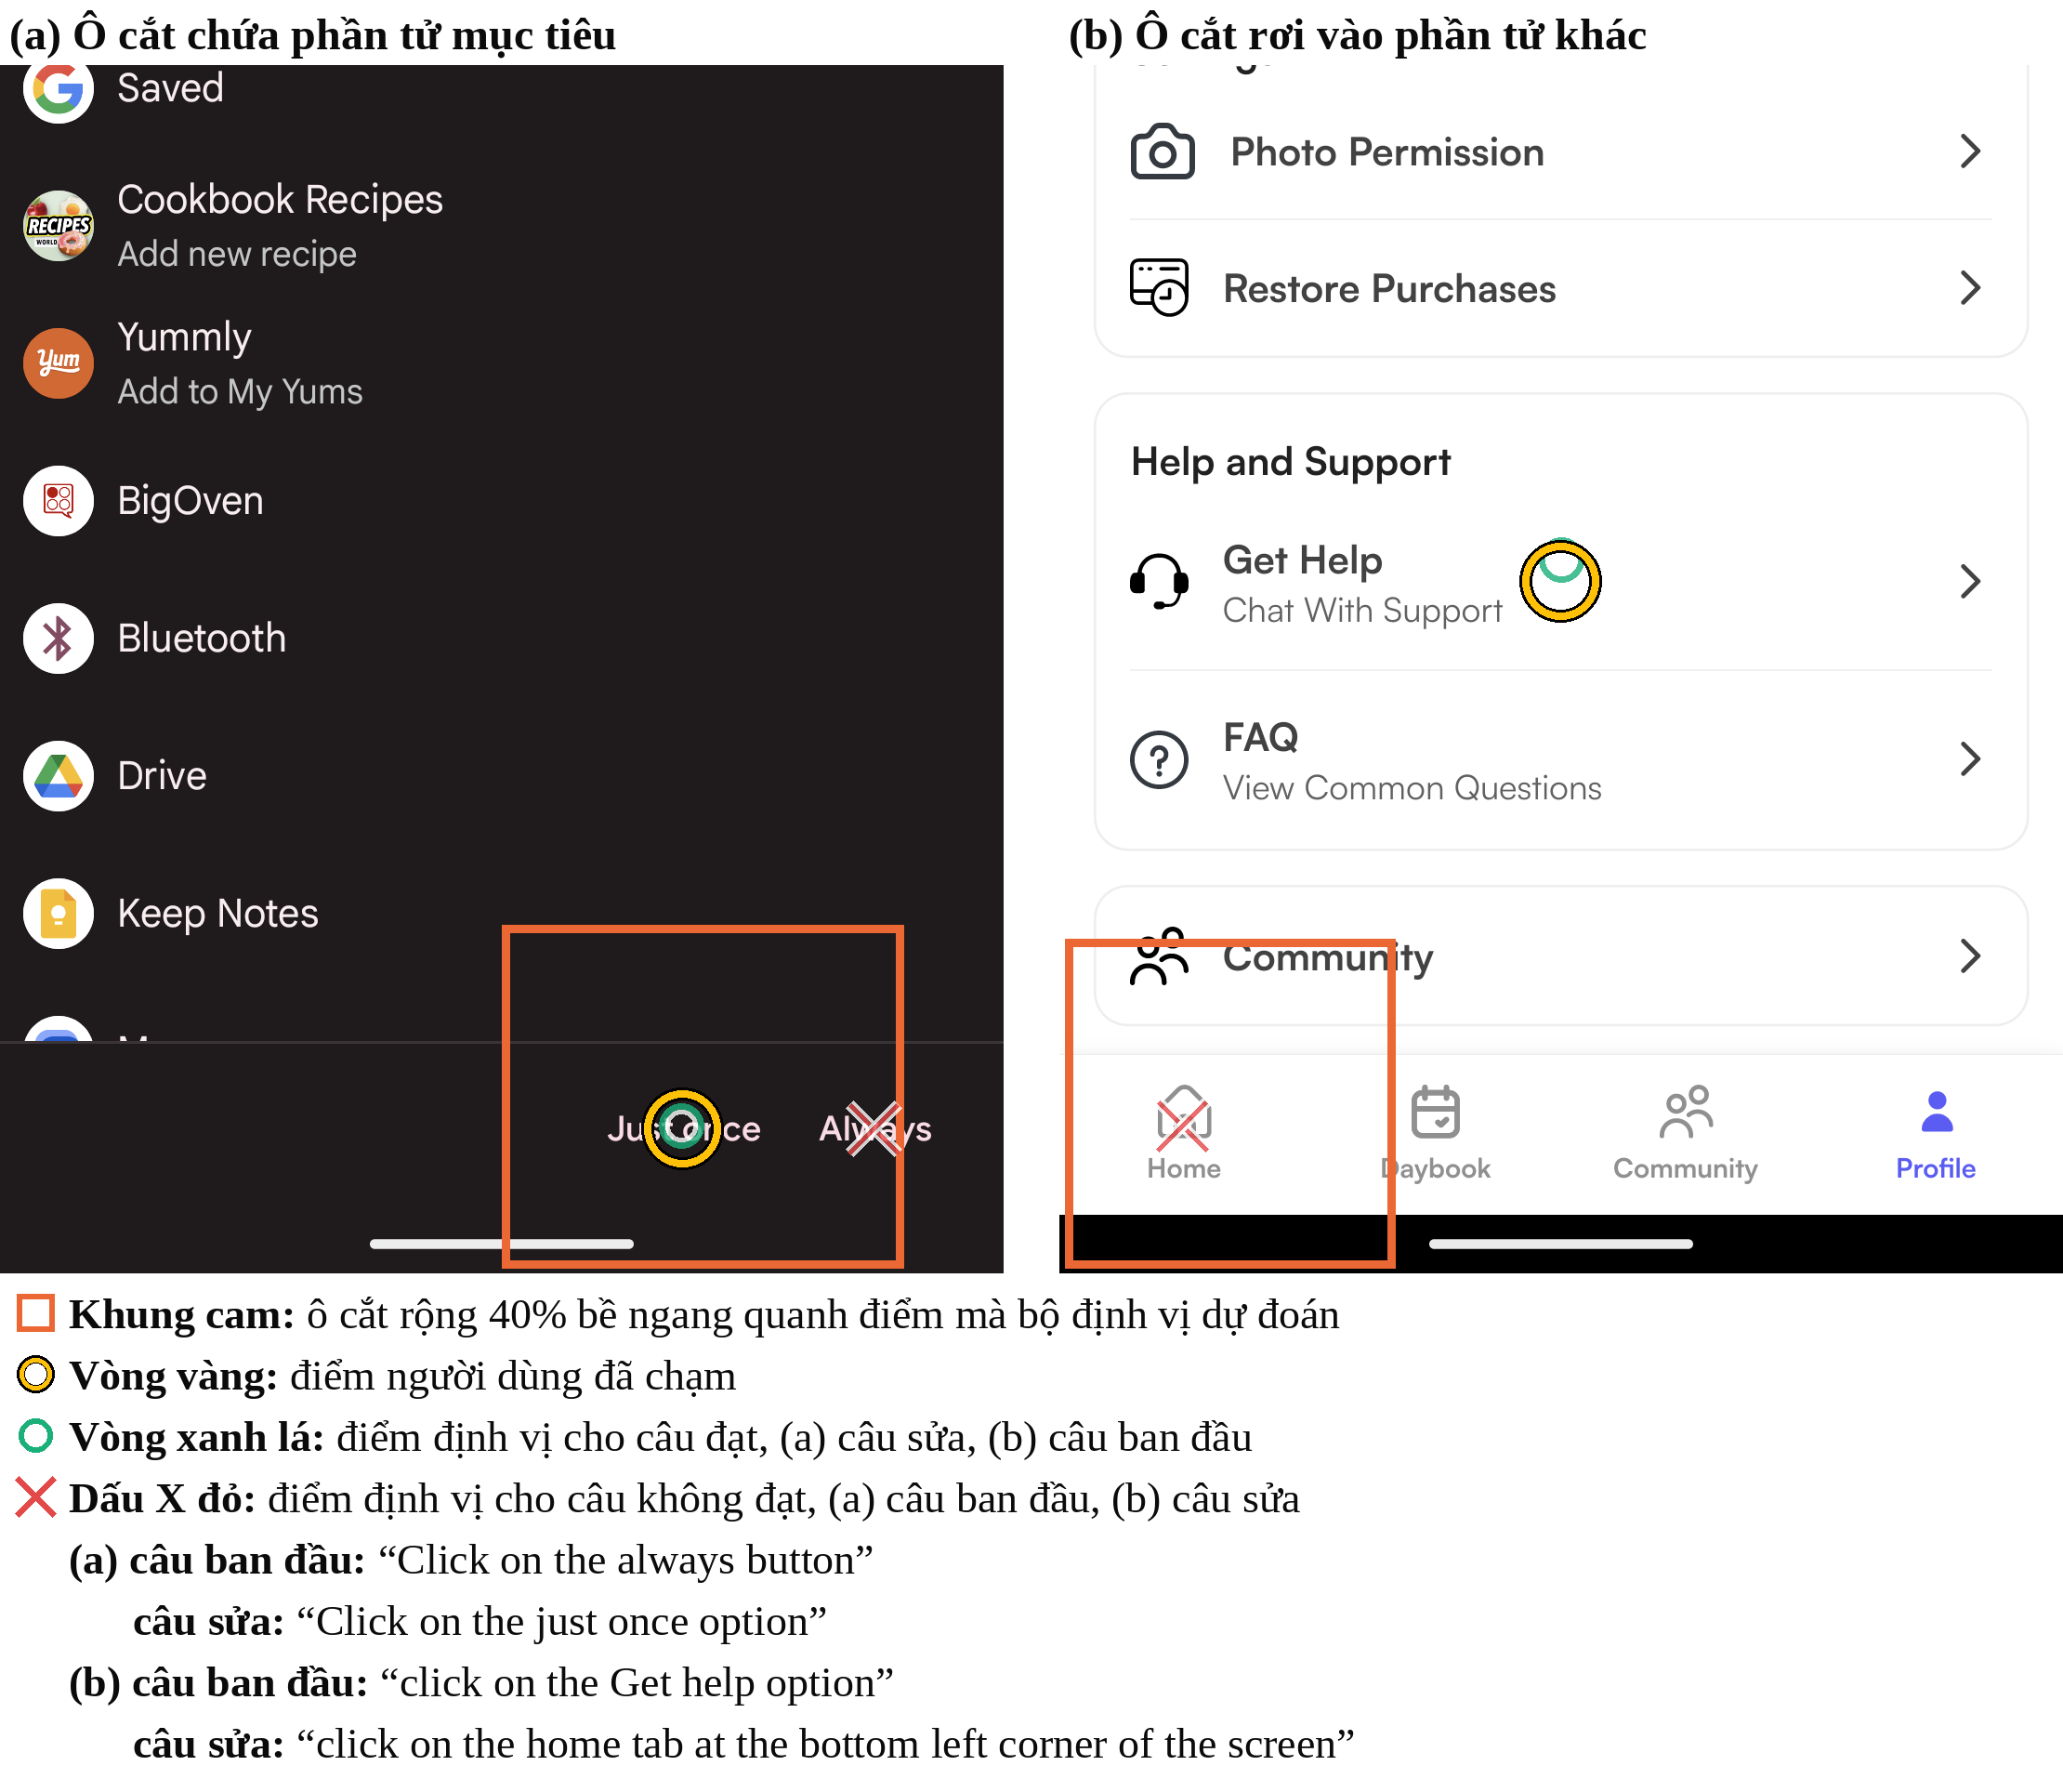
\includegraphics[width=\textwidth]{figures/fig_vidu_tage.png}
\caption[Hai bước mà bộ chọn của TAGE nhận câu sửa, cắt phần dưới màn hình.]{Hai bước mà bộ chọn của TAGE nhận câu sửa, cắt phần dưới màn hình. (a) Ô cắt đúng chỗ: câu nháp gọi nút \emph{Always}, câu sửa gọi đúng \emph{Just once}. (b) Ô cắt rơi vào thanh điều hướng ở góc dưới bên trái: câu nháp \emph{Get help} vốn đúng bị thay bằng câu về thẻ \emph{Home} nằm trong ô cắt.}
\label{fig:A.2}
\end{figure}

\textbf{Tín hiệu của bộ chọn.} Theo Hình~\ref{fig:A.3}, tỉ lệ ô cắt đúng chỗ giảm đều khi $\Delta$lp tăng, từ 74,0\% ở nhóm thấp nhất xuống 36,5\% ở nhóm được nhận. Cách đọc khả dĩ là khi ô cắt rơi vào phần tử khác, bộ biên tập viết một câu rất chắc chắn về phần tử trong ô, còn câu nháp nói về phần tử ngoài ô nên bị đánh giá log-xác suất thấp. Hiệu $\Delta$lp vì vậy đo mức lệch giữa câu nháp và ô cắt, và không cho biết câu nào đúng hơn. Trên tập kiểm định nội bộ, nhóm trên cùng chỉ có 11 câu và tình cờ có 8 ô cắt đúng chỗ, mà $\tau$ lại được chọn từ chính 11 câu ấy.

\begin{figure}[t]
\centering
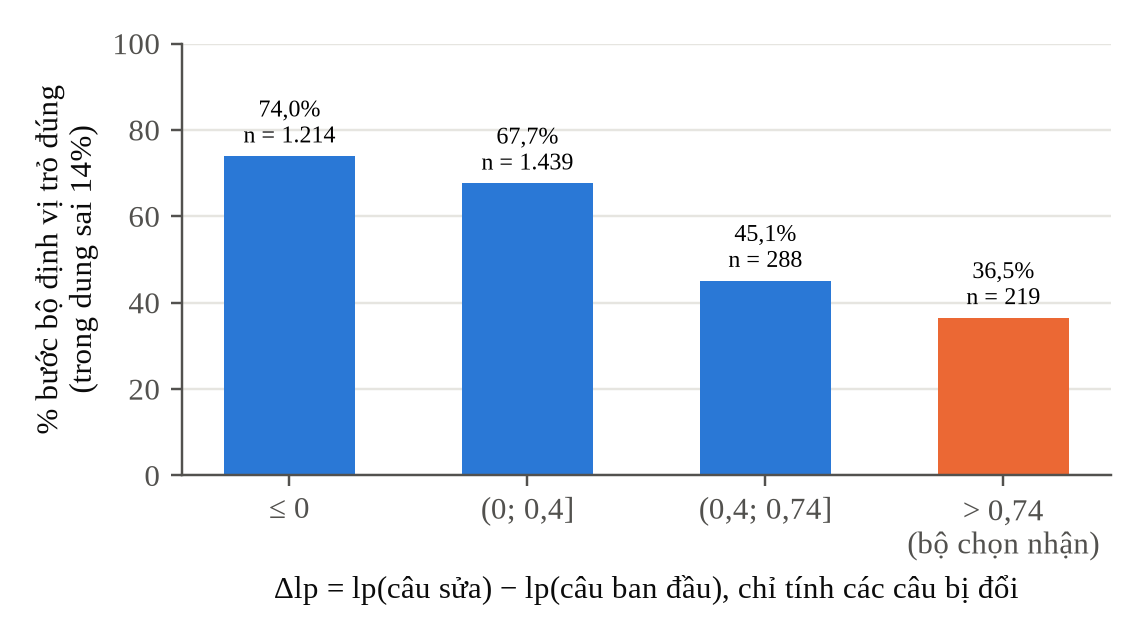
\includegraphics[width=0.82\textwidth]{figures/fig_tage_cong.png}
\caption[Tỉ lệ ô cắt đúng chỗ (bộ định vị trỏ trong dung sai 14\%) theo nhóm $\Delta$lp, trên các câu mà bộ biên tập đã đổi ở tập kiểm tra.]{Tỉ lệ ô cắt đúng chỗ (bộ định vị trỏ trong dung sai 14\%) theo nhóm $\Delta$lp, trên các câu mà bộ biên tập đã đổi ở tập kiểm tra. Cột cam là nhóm được nhận. Bộ chọn càng tự tin nhận câu sửa thì ô cắt càng hay sai.}
\label{fig:A.3}
\end{figure}

\textbf{Hệ quả cho thiết kế.} Bộ chọn dựa trên xác suất của chính bộ biên tập không độc lập với ô cắt, nên không bắt được lỗi nguy hiểm nhất của bộ sửa câu là ô cắt sai. Bộ chọn cần một tín hiệu không đi qua ô cắt, ví dụ so điểm mà mô hình định vị trỏ theo câu nháp với điểm của bộ định vị, và $\tau$ cần được chọn trên mẫu lớn hơn nhiều so với 11 câu. Nếu bộ chọn chỉ nhận câu sửa khi ô cắt đúng chỗ, bộ sửa câu được thêm 39 bước, khoảng 0,87 điểm. Đây là ngưỡng tối đa ước lượng bằng điểm chạm đúng của bước, không phải kết quả của một cấu hình đã chạy.

